\section{Aufbau}
\label{sec:Aufbau}
Ein Schaltbild des Versuchsaufbaus ist in \autoref{fig:Schaltbild} dargestellt. 
\begin{figure}[H]
    \centering
    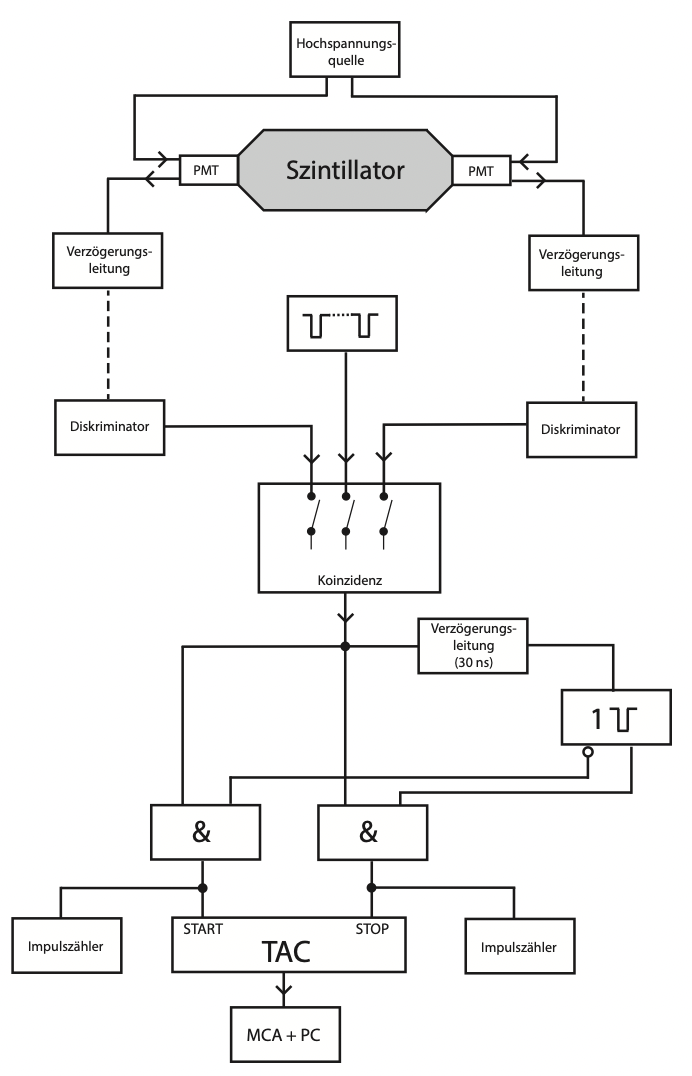
\includegraphics[width=0.5\textwidth]{Abbildungen/Schaltung.png}
    \caption {Schematische Dastellung des Versuchsaufbaus.\cite{V01}}
    \label{fig:Schaltbild}
\end{figure}
Dabei besteht der Versuchsaufbau aus einem Szintillatortank, welcher ein Volumen von ungefähr $\qty{50}{\liter}$ fasst.
An beiden Ausgängen des Szintillatortanks ist je ein Photomultiplier (PMT) gekoppelt, welcher schwache Lichtsignale durch Erzeugung und Verstärkung eines elektrischen Signals detektiert.
Dessen Ausgänge werden über eine Verzögerungsleitung auf den den Eingang eines Diskriminators gegeben, welcher eine variable Schwelle besitzt. 
Anschließend gelangen die Signale beider PMT in eine Koinzidenzschaltung, welche nur dann ein Ausgangssignal erzeugt, wenn beide Signale der PMT zeitgleich an den Eingangen der Koinzidenzschaltung
eintreffen.\\
Danach folgt das elektronische Äquivalent einer Stoppuhr.
Das Ausgangsignal der Koinzidenzschaltung gelangt zu zwei AND-Gattern und über eine weitere Verzögerungsleitung ($\qty{30}{\nano\second}$) zu einem Monoflop. Dieser gibt die Suchzeit $T_S$ vor.
Aufgrund der Verbindung der AND-Gitter mit dem Time-Amplitude-Converter (TAC), startet die Zeitessung durch das Signal des ersten AND-Gatters,
wenn ein Myon das aktive Volumen betritt. Die Zeitmessung stoppt aufgrund eines Signal des anderen AND-Gatters, wenn das Myon zerfällt. 
Außerdem wird sie Zeitmessung bzw. der Monoflop zurückgesetzt wenn die Suchzeit $T_S$ abgelaufen ist, ohne dass ein Stoppsignal ausgelöst wurde.
Die Start- und Stoppimpulse werden gezählt, indem die Gatter außerdem jeweils mit einem Impulszähler verbunden sind.
Das Signal des TAC gelangt zu einem Vielkanalanalysator (bzw. Multi-Channel-Analyser) (MCA). Dieser ordnet jedem Signal entsprechend
seiner Größe einen Kanal innerhalb eines Datensatzes zu und erhöht den Wert des entsprechenden Kanals um Eins. Die Anzahl der in einem Kanal
gespeicherten Signale entspricht also der Häufigkeit des Auftretens eines Signals mit einer bestimmten Lebensdauer. Das Histogramm der
Kanäle kann am PC durch eine bestimmte Messsoftware augelesen werden.


\subsection{Rauschunterdrückung}
\label{subsec:Rauschunterdrückung}
Bei endlichen Temperaturen neigen Photokathoden zu spontaner Elektronemission, wobei kleine Impulse entstehen.
Diese Impulse sind kleiner als "echte" Impulse und können so mit einem Diskriminatoren rausgefiltert werden. Die Schwelle wird
dabei so gesetzt, dass möglichst nur die ungewollten Impulse rausgefiltert werden. Es kann jedoch dazu kommen, dass auch "echte"
Impulse rausgefiltert werden, weswegen auf beiden Seiten ein PMT mit Diskriminator angeschlossen wird. 
So dass wenn ein Myon eintrifft und zerfällt beide PMT das Signal aufnehmen und zur Koinzidenz weiterleiten.

\subsection{Stoppuhr-Methode}
\label{subsec:Messmethode}
Es kann sein, dass Myonen in den Szintillator gelangen und dann entweder von dem Szintillator absorbiert werden oder sie genug 
Energie haben um durch das Szintillatormaterial und den Detektor zu bewegen. Bei beiden Fällen kann nicht die Lebenszeit von Myonen bestimmt werden.
Es wird somit von diesen Myonen nur ein Impuls gesendet und der Impuls des nächsten eintreffenden Myons würde als Zerfallsimpuls des ersten
registriert werden. Um dagegen zu wirken
wird die Stoppuhr-Methode benutzt. Dabei beginnt eine Suchzeit $T_S$ nach dem Startimpuls. Zerfällt das Myon nicht innerhalb der Suchzeit,
wird die Apparatur wieder in den Anfangszustand zurückgebracht.\\
Diese grundlegende Messprinzip wird schaltungstechnisch durch den Monoflop und den zwei AND-Gittern geregelt.
Der Monoflop hat einen stabilen und einen instabilen Zustand.
Die Zeit, in der der Monoflop im instabilem Zustand ausglenkt ist, sollte ungefäht der Suchzeit eintsprechen, weil im stabilen Zusatnd sendet
der Monoflop ein Signal an das zweite AND-Gitter, was die Messung stoppt.
Die Koinzidenzschaltung lenkt dabei den Monoflop in den instabilen Zustand aus und das TAC misst die Zeit. Kommt es dann in der Suchzeit zu keinem
Stromimpuls, der über das zweite AND-Gatter an das TAC weitergeleitet wird, wird die Messung verworfen und das TAC gibt kein Signal ab.
Um die Anzahl der verworfenen Messungen zu bestimmen, wird ein weiterer Impulszähler angeschlossen.\\
Treffen zwei Myonen gleichzeitig innnerhalb der Suchzeit im Tank ein, kommt es zu einer Fehlermessung, die auch Untergrund genannt wird.
Dabei ist der Zeitabstand in dem zwei Myonen eintreffen statistisch verteilt und füllt daher die Kanäle des Vielkanalanalysator gleichmäßig auf.

\section{Durchführung}
\label{sec:Durchführung}
Für die Durchführung des Versuchs wird die Schaltung wie in \autoref{sec:Aufbau} aufgebaut und  anschließend kalibriert.
Dabei wird zur Überprüfung der Schaltung ein Oszilloskop benutzt.\\
Zur Einstellung der Schwellspannung der Diskriminatoren, werden zunächst die Spannungsimpulse der Photomultiplier mit dem Oszilloskop überprüft.
Die Spannungsimpulse sollten vor den Diskriminatoren von unterschiedlicher Höhe und Länge sein und die Diskriminatorschwelle wird so eingestellt,
dass an beiden Ausgängen ungefähr $30$ Impulse pro Sekunde gemessen werden, welche nun die gleiche Höhe besitzen.
Die Pulsdauer wird auf $\Delta t = \qty{10}{\nano\second}$ eingestellt, was klein gegenüber der Lebensdauer der Myonen ist, damit sich zwei Impulse
möglichst nicht überlagern.\\
Anschließend wird der Koinzidenzschaltung eingestellt, indem die Verzögerungsleitungen so gewählt werden, dass die Signale gleichzeitig eintreffen. Dabei wird der Messbereich so gewählt,
dass sich die Halbwertsbreite der Verteilung bestimmen lässt. Die Ereignisrate soll im Bereich von $\qty{20}{\second^{-1}}$ liegen.\\
Danach wird der restliche Teil der Schaltung verkabelt, eine Suchzeit $T_S$ eingestellt und der Messbereich des TAC entsprechend angepasst.
Der MCA kann über einen Doppelimpulsgenerator kalibriert werden. Dieser Doppelimpulsgenerator generiert dabei Doppelimpulse mit einem
variablen Zeitabstand bei einer Frequenz von $\qty{1}{\kilo\Hz}$. Die Kalibration wird für zehn Messwerte im Bereich von
$\qty{0.3}{\micro\second}$ bis $\qty{9.9}{\micro\second}$ durchgeführt. Dabei wird bei allen Messpunkten die gleiche Messzeit benutzt
und anschließend die absolute Zählrate verglichen.
Um die verfügbaren Kanäle des Vielkanalanalysators optimal ausnutzen zu können wird die Spannungsausgabe des
TAC so eingestellt, dass bei Impulsabständen von $\qty{9.9}{\micro\second}$ ungefähr der mittlere Kanal
aufgefüllt wird.\\
Nach erfolreicher Kalibration werden die Photomultiplier angeschlossen und die eigentlich Messung beginnt.
Dabei werden die individuellen Lebensdauern der Myonen für ?? Stunden aufgenommen und als Histogramm dargestellt.
Aus dem Histogramm wird dann die mittlere Lebensdauer der Myonen bestimmt.


